\documentclass[12pt, twoside]{article}
\usepackage{jmlda}
\newcommand{\hdir}{.}

\renewcommand{\baselinestretch} {1.35}
\usepackage{xcolor}

\usepackage[english, russian]{babel}
\usepackage[utf8]{inputenc}

\usepackage{graphicx}
\usepackage{caption}
\usepackage{subfig}
\graphicspath{{phase/}}
\DeclareGraphicsExtensions{.pdf,.png,.jpg}

\usepackage[usenames]{color}
\usepackage{colortbl}

\newcommand{\N}{\mathbb{N}}
\newcommand{\Z}{\mathbb{Z}}

\theoremstyle{definition}

\newenvironment{theorem}[2][Теорема]{\begin{trivlist}
\item[\hskip \labelsep {\bfseries #1}\hskip \labelsep {\bfseries #2.}]}{\end{trivlist}}
\newenvironment{lemma}[2][Lemma]{\begin{trivlist}
\item[\hskip \labelsep {\bfseries #1}\hskip \labelsep {\bfseries #2.}]}{\end{trivlist}}
\newenvironment{exercise}[2][Задача]{\begin{trivlist}
\item[\hskip \labelsep {\bfseries #1}\hskip \labelsep {\bfseries #2.}]}{\end{trivlist}}
\newenvironment{reflection}[2][Reflection]{\begin{trivlist}
\item[\hskip \labelsep {\bfseries #1}\hskip \labelsep {\bfseries #2.}]}{\end{trivlist}}
\newenvironment{proposition}[2][Proposition]{\begin{trivlist}
\item[\hskip \labelsep {\bfseries #1}\hskip \labelsep {\bfseries #2.}]}{\end{trivlist}}
\newenvironment{corollary}[2][Corollary]{\begin{trivlist}
\item[\hskip \labelsep {\bfseries #1}\hskip \labelsep {\bfseries #2.}]}{\end{trivlist}}


\def\eps{\varepsilon}
\def\T{{\cal T}}
\def\H{{\cal H}}
\def\K{{\cal K}}
\def\L{{\cal L}}
\def\F{{\cal F}}
\def\Q{{\cal Q}}
\def\N{{\cal N}}
\def\p{{\cal P}}
\def\np{{\cal NP}}
\def\A{{\cal A}}
\def\B{{\cal B}}
\def\D{{\cal D}}
\def\BB{{\cal B}^* }
\def\DD{{\cal D}^* }
\def\TT{\tilde{\cal T}}
\def\f{\tilde f}
\def\ind{\mathop{\rm index}}
\def\St{\mathop{\rm St}}
\let\bd\partial
\def\V{\ensuremath{{\cal V}}}
\def\SS{{\mathbb S}}
\def\RR{\mathbb R}
\def\QQ{\mathbb Q}
\def\PP{\mathbb P}
\def\AA{\mathbb A}
\def\R{\cal R}
\def\NN{\mathbb N}
\def\CC{\mathbb C}
\def\ZZ{\mathbb Z}
\def\s{\sigma}
\def\S{\Sigma }
\def\ss{\Sigma^* }
\def\ra{\rightarrow}
\def\da{\downarrow}
\def\Ra{\Rightarrow}
\def\t{\theta}

\begin{document}

\title
    [] % краткое название; не нужно, если полное название влезает в~колонтитул
    {Detection of phase and change point of human motions with signals of wearable devices}
\author
    [A.\,D.~Kurdyukova] % список авторов (не более трех) для колонтитула; не нужен, если основной список влезает в колонтитул
    {A.\,D.~Kurdyukova, G.\,V.~Kormakov, D.\,M.~Tihonov, V.\,V.~Strijov} % основной список авторов, выводимый в оглавление
    [A.\,D.~Kurdyukova, G.\,V.~Kormakov, D.\,M.~Tihonov, V.\,V.~Strijov] % список авторов, выводимый в заголовок; не нужен, если он не отличается от основного
\email
  {kurdiukova.ad@phystech.edu; egor2898@mail.ru; tihonov.dm@phystech.edu;  strijov@ccas.ru}
%\thanks
%    {Работа выполнена при
%     %частичной
%     финансовой поддержке РФФИ, проекты \No\ \No 00-00-00000 и 00-00-00001.}
%\organization
%    {$^1$Организация, адрес; $^2$Организация, адрес}
\abstract
  {The paper proposes detections of the phase and check point of human motions. \emph{Signals of wearable devices. Human motion is quasi-periodic.} Find the phase of quasi-periodic movement. Determine the moment of changing the type of movement. For this purpose, the author proposes to solve the task of segmenting time series. In this paper we construct the phase trajectory of the motion and find the actual dimension of the phase space. The proposed model estimates the phase of motion and determines the beginning of the segment. Repeat of the phase trajectory enable to segment the periodic actions of a person. Change point enable to determine a change in the type of movement. The computational experiment analyzes the quality of the proposed model. The time series are collected from the three-axis accelerometer.

\bigskip
\noindent
\textbf{Keywords}: \emph {time series, phase trajectory, trajectory space, segmentation, disorder, principal component analysis}
}

%данные поля заполняются редакцией журнала
\doi{}
\receivedRus{}
\receivedEng{}

\maketitle
\linenumbers

\newpage

\title
    [] % краткое название; не нужно, если полное название влезает в~колонтитул
    {Определение фазы и разладки движения человека по сигналам носимых устройств}
\author
    [А.\,Д.~Курдюкова] % список авторов (не более трех) для колонтитула; не нужен, если основной список влезает в колонтитул
    {А.\,Д.~Курдюкова, Г.\,В.~Кормаков, Д.\,М.~Тихонов, В.\,В.~Стрижов} % основной список авторов, выводимый в оглавление
    [А.\,Д.~Курдюкова, Г.\,В.~Кормаков, Д.\,М.~Тихонов, В.\,В.~Стрижов] % список авторов, выводимый в заголовок; не нужен, если он не отличается от основного
\email
   {kurdiukova.ad@phystech.edu; egor2898@mail.ru; tihonov.dm@phystech.edu;  strijov@ccas.ru}
%\thanks
%    {Работа выполнена при
%     %частичной
%     финансовой поддержке РФФИ, проекты \No\ \No 00-00-00000 и 00-00-00001.}
%\organization
%    {$^1$Организация, адрес; $^2$Организация, адрес}
\abstract
  {Данная работа посвящена определению фазы и разладки движения человека по сигналам носимых устройств. Исследуются несколько классов периодического движения человека. Требуется построить модель, которая восстанавливает фазу движения, а также определить момент смены типа движения. Строится фазовая траектория движения и отыскивается фактическая размерность фазового пространства. По разладке фазовой траектории определяется смена типа движения. Качество предлагаемой модели анализируется на временных рядах, считанных с трехосевого акселерометра.

\bigskip
\noindent
\textbf{Ключевые слова}: \emph {временные ряды, фазовая траектория, траекторное пространство,  сегментация, разладка, метод главных компонент}
}

%данные поля заполняются редакцией журнала
\doi{}
\receivedRus{}
\receivedEng{}

\maketitle
\linenumbers

\section{Введение}
Решается задача анализа сигналов, считываемых с носимых устройств. Результаты анализ этих данных используются в различных медицинских приложениях \cite{bussmann1998ambulatory, najafi2003ambulatory}, в частности, при мониторинге состояния пациентов \cite{grunerbl2014smartphone}, для автоматизированного обнаружения падений пожилых людей \cite{ma2014depth}.

Временной ряд $\{s_t\}_{t=1}^N$\, движения человека назовем \emph{квазипериодическим} с периодом $T$, если для всех $t\in[0,+\infty)\,$ найдется $\delta$, такое что для любого $l\in\NN\,$ выполнено
    \begin{equation}\label{st}
       s_{t} \approx s_{t + lT + \delta}, \quad |\delta| \ll T.
    \end{equation}
% Решается задача разбиения временных рядов на квазипериодические временные интервалы. Целью этой работы является построение модели $f$ фазовой траектории и моедли определения фазы
%     \begin{equation}\label{model}
%         g(v):\: t\; \rightarrow\; \varphi. 
%     \end{equation}

При анализе временных рядов рассматривают разбиения (такие разбиения называются сегментацией или класетризацией []) на квазипериодические временные интервалы, которые позволяют перейти в пространство фазовых траекторий. 

Предлангается способ оценки фиксированной размерности собственного подпространства фазовых траекторий. В работах \cite{motrenko2015extracting, grabovoy2020quasi, usmanova} показана избыточность исходного пространства для построения аппроксимирующей модели. Она восстанавливает временной ряд по фазовым траекториям в собственном подпространстве. адекватно приближая исходный квазипериодический временной ряд~\eqref{st}. 

  \begin{figure}[ht]\label{fig1}
            \center{\includegraphics[scale = 0.165]{phase2.jpg}}
            \caption{Фазовая траектория временного ряда \eqref{st}}
    \end{figure}

Для сегментации квазипериодических временных рядов необходимо определить период. 
%повторения некоторого значения, в пространстве фазовых траекторий, с точностью до допустимой ошибки фиксированной величины.%
\emph{Ввести определение фазы?}
Данное значение фазовой траектории интерпретируется как начальная фаза фиксированного класса. В собственном подпространстве возможно более устойчивое извлечение начальной фазы. При добавлении шума в исходный временной ряд модель, определяющая фазу, не изменяет существенно своего прогноза.   

В работах \cite{motrenko2015extracting, ignatov2016human}  решается задача сегментации квазипериодических временных рядов. Переход в собственное подпространство фиксированной размерности, равной двум, является сильным ограничением. Данное предположение на размерность опирается на теорему~\cite{motrenko2015extracting} об аппроксимации периодических компонент синусоидального временного ряда с периодом~$T > 2$. В реальных данных встречается суперпозиция нескольких главных компонент, для которых эта теорема неприменима. Размерность собственного подпространства, равная двум, не является достаточной для построения устойчивой модели.

В работах \cite{ignatov2016human, grabovoy2020quasi} задача сегментации квазипериодических временных рядов решается путем построения низкоразмерного фазового пространства и переходом к признаковому описанию точек исходного временного ряда с использованием метрик в фазовом пространстве. При работе в высокоразмерном фазовом пространстве данный подход становится более неустойчивым из-за ''проклятия размерности''. 

Целью данной работы является построение алгоритма нахождения устойчивой фазы квазипериодического временного ряда. Предлагаемый алгоритм прогнозирует фазу временного ряд фиксированного класса  периодического движения. \emph{в пространстве оптимальной размерности.} Описывается критерий оптимальности размерности, опирающийся на условие отсутствия самопересечений в фазовом пространстве.

% Целью данной работы является переход в фазовое пространство минимальной размерности. \emph{Фазовая траектория не имеет самопересечений с точностью до стандартного отклонения восстановленной траектории}.

\section{Постановка задачи}
Данные, считанные с трехосевого акселерометра с частотой семплирования $\nu = 500 c^{-1}$, представляют собой временной ряд 
    \begin{equation}\label{ts_3}
        \{ \mathbf{a}_i \}_{i = 1}^{N}, \quad \mathbf{a}_i = \begin{bmatrix}a_{ix}\;a_{iy}\;a_{iz}\end{bmatrix}^{\mathst{T}},\quad \mathbf{a}_i \in \RR^3.
    \end{equation}
В работе рассматривается временной ряд
    \begin{equation}\label{ts}
        \{ s_i \}_{i = 1}^{N}, \quad s_i = \sqrt{a_{ix}^2 + a_{iy}^2 + a_{iz}^2},\quad s_i \in \RR^1.
    \end{equation}    
Предполагается, что он соответствует фиксированному классу периодического движения~ $y\in\mathbb{Y}:\:$ходьба, бег, шаги вверх или вниз по лестнице. Для анализа периодических компонент осуществляется переход в собственное пространство с проомощью построения ганкелевой матрицы. Далее в текущей работе будем называть ее траекторной матрицей.

Временной ряд \eqref{ts} представлен в виде разложения, каждое слагаемое которого аппроксимируется комбинацией главных компонент траекторной матрицы
    \[ \mathbf{H} = \begin{bmatrix}
                        s_1 & \dots & s_n \\
                        s_2 & \dots & s_{k+1} \\
                        \hdotsfor{3} \\
                        s_{N-n+1} & \dots & s_N
                    \end{bmatrix}^\top = \begin{bmatrix}
                        \mathbf{s}_1 \\
                        \mathbf{s}_2  \\
                        \hdotsfor{1} \\
                        \mathbf{s}_m 
                    \end{bmatrix}^\top, \quad m = N - n + 1 \]
где~$n$ -- ширина окна, не меньшая, чем преполагаемый период: $n\mu^{-1} \leq T$ 
Для понижения размерности фазового пространства выполняется сингулярное разложение матрицы $\mathbf{H}^\top\mathbf{H}$
    \[ \frac{1}{n}\mathbf{H}^{\mathsf{T}}\mathbf{H} = \mathbf{V}\mathbf{\Lambda}\mathbf{V}^{\mathsf{T}}, \quad \mathbf{\Lambda} = \diag(\lambda_1,\dots,\lambda_{n}). \]
    после чего определяются главные компоненты $\mathbf{y}_k = \mathbf{Hv}_k,\, k\in \overlin{1, \dots, n}$ для ее собственных значений.

Требуется построить модель $f$, аппроксимирующую фазовую траекторию с помощью минимального числа главных компонент. Предполагается, что траектория порождает движение человека из фиксированного класса. Каждая модель аппроксимирует временной ряд заданного класса $y$. На рисунке () изображено ? сегмента класса ходьбы 
   

Размерность исходного фазового пространсства избыточна. Осуществляется переход в собственное подпространство меньшей размерности. Пусть $\mathbf{y}_1,\dots,\mathbf{y}_p$ -- выбранные главные компоненты, аппроксимирующие фазовую траекторию. Восстановленная часть траекторной матрицы $\mathbf{\widehat{H}}$
    \[ \mathbf{\widehat{H}} = \mathbf{H}_1  + \dots + \mathbf{H}_p, \quad \mathbf{H}_j = \sqrt{\lambda_j}\mathbf{v}_j\mathbf{y}_j^{\mathsf{T}},\quad j\in\overline{1, p}\]
    \[ \mathbf{X} = \mathbf{\widehat{H} W} = \begin{bmatrix}
                        \mathbf{x}_1 \\
                        \mathbf{x}_2  \\
                        \hdotsfor{1} \\
                        \mathbf{x}_m 
                    \end{bmatrix}, \quad \mathbf{x}_i\in \RR^p, \,  \]
где $\mathbf{W}$ --- матрица преобразования алгоритма PCA с количеством компонент равным $p$, соответствующим наибольшим собственным значениям.

В полученном фазовом пространстве требуется построить модель фппроксимации фазовой траектории, определить критерий выбора оптимальной размерности пространства и модель нахождения фазы в исходном временном ряде.
% С помощью антидиагонального усреднения матрицы $\mathbf{\widehat{H}}$ восстанавливается временной ряд~\eqref{ts}. Критерием качества аппроксимации является MAPE, средняя абсолютная процентная ошибка
%     \[ \text{MAPE} = \frac{1}{N}\sum_{i = 1}^{N}100\frac{|\hat{x}_i - x_i|}{|x_i|}. \]


    % \begin{figure}[ht]\label{fig2}
    %         \center{\includegraphics[scale = 0.165]{phase1.jpg}}
    %         \caption{}
    % \end{figure}

\section{Определение фазы в пространстве оптимальной размерности}
\subsection{Аппроксимационная модель фазовой траектории}
Из предыдущего раздела найдена модель $f$, переводящая исходный временной ряд в фазовое пространство.   
Обозначим за $g: \varphi \rightarrow \mathbf{x}$ модель, ставящую в соответствие фазе $\varphi \in [0, 2\pi]$ точки средней траектории $\Expect(\mathbf{x}|\varphi)$ и дисперсии $\Variance(\mathbf{x}|\varphi), \; \mathbf{x}\in\RR^p$. 

Аппроксимационная модель $g^{-1}$ сопоставляет точке собственного  подпространства размерности~$\mathbf{x}_i\in\RR^p$ скалярную величину $\varphi_i\in[0,2\pi], \; i\in\overline{1, m}$. Таким образом, общая схема выглядит следующим образом
\begin{equation}\label{eq:g}
t_i \xrightarrow{f} \mathbf{x}_i \xrightarrow{g^{-1}(\mathbf{x}_i)} \varphi_i ,\end{equation}
где $ t_{i+1} = t_i + T\nu^{-1},\; t_0 = 0$ -- удар каблука.

Модель~$g$ используется для получения точек~$\mathbf{x}_i$ по фазе.
Предлагается осуществить аппроксимацию по траекторной матрице $\mathbf{X}$ с помощью регрессии Надарая-Ватсона.
Тогда средняя траектория получается по формуле
    \begin{equation}\label{eq:NW}            
    \Expect(\mathbf{x}_i|\varphi) =\frac{\sum_{\mathbf{x}_i\in X}\mathbf{x}_iK\left(\frac{\rho(\varphi', \varphi)}{h}\right)}{\sum_{\mathbf{x}_i\in X}K\left(\frac{\rho(\varphi', \varphi)}{h}\right)},  \end{equation}
где $h$ -- фиксированная ширина окна, $\varphi'$ -- предполагаемые фазы точек фазовой траектории $\mathbf{X}$ .
При помощи имеющихся предположений о периоде $T$ сопоставляем каждой точке фазовой траектории фазу $\varphi'  = \frac{2\pi \cdot i}{T} \mod 2\pi$.

В качестве ядра предлагается рассмотреть следующие функции спользуется RBF функция
    \[ K(r)= \exp\left(-\gamma\| r \|^2\right) \text{ -- RBF функция}\]
       \[\text{П}(r) = [|r|\leq 1] \text{ -- прямоугольое ядро}\]
      \[ T(r) = (1 - |r|)[|r|\leq 1] \text{ -- треуголное ядро}\]
      \[ E(r) = (1 - |r|^2)[|r|\leq 1] \text{ -- квадратичное ядро}\]
Введена метрика
    \[ \rho(\varphi', \varphi) = \frac{1 - \cos(\varphi' - \varphi)}{2}, \quad \varphi',\, \varphi \in [0, 2\pi]\]
Соответствующие значения дисперсии
    \[  \Variance(\mathbf{x}_i|\varphi) = \dots, \quad i\in \overline{1, T}  \]

\subsection{Обнаружение самопересечений}
 \textbf{Определение.}
 Оптимальная размерность пространства - это размерность пространства, в которой выполняется критерий
отсутствия самопересечений 
 
Введем множество индексов
    \[ M = \left\{ i\,|\, \Expect(\mathbf{x}_i|\varphi)\pm\Variance(\mathbf{x}_i|\varphi)\bigcap\Expect(\mathbf{x}_j|\varphi)\pm\Variance(\mathbf{x}_j|\varphi)\neq\varnothing, \; \mathbf{x}_j\in X,\; |i - j| > k
    \right\},\;k\in\NN, \, k\geq \frac{T}{4} \]
Если множество $M$ пусто, то самопересеений нет. 

\subsection{Модель определения фазы}

% Пусть мы находимся в пространстве достаточной размерности.\\ Модель $g(v)$ для любой точки фазовой траектории $\mathbf{x}_i\rightarrow \varphi_i \in [0,2\pi]$.


% \textcolor{Gray}{Умеем определять фазу для точек средней траектории. Как определить фазу произвольной точки $\mathbf{x}_i$ на фазовой траектории? Так как отсутствуют самопересечения, то берем точки средней фазовой траектории $\{ \mathfrac{x}_j\}_{j = 1}^k$, в область дисперсии которых попадает $\mathbf{x}_i$, и считаем среднее значение фазы
%     \[ \mathbf{x}_i \rightarrow \varphi_i = \frac{\sum_{j = 1}^k\mathrfac{\varphi}_j}{k}. \]
% Критерий качетсва, хорошо ли работает модель. Нет минимизации функции потерь.}

% Выбранная модель
%     \[ \varphi \xrightarrow{g(v)} \mathrm{E}(v|\varphi),\, \mathrm{D}(v|\varphi).  \]

%  В рамках данной работы предлагается увеличить число точек средней траектории (и соответствующей дисперсии) с помощью интерполяции. В результате, для текущей точки фазовой траектории алгоритм будет корректнее находить ближайших соседей.

Для определения фазы модель опирается на следующие предположения
\begin{enumerate}
    
    \item Точкам с большим индексом соответствует большая фаза.  
    Если $j > i$, то $\varphi_j > \varphi_i$ для~$i,\, j \in \overline{1, m}$.
    
    \item Фазы соседних точек близки. Если $\| \mathbf{x}_i - \mathbf{x}_j \|_2^2 < \eps$ ($\eps$ -- гиперпараметр), то $\| \varphi_i - \varphi_j \| < \delta$ для некоторого $\delta$, где $i,\, j \in \overline{1, m}$.
\end{enumerate}

% (соседние $x_i\rightsquigarrow x_j$)
\emph{Выбор предполагаемых фаз.}
% Для определения фазы текущей точки и опираясь на эти предположения задается По этим предположениям формируется множество 
Для каждой точки фазовой траектории (?) введем множество индексов точек средней траектории, попадающих в область дисперсии \[N_i = \{ j\,|\, \mathbf{x}_i\in\Expect(\mathbf{x}_j|\varphi)\pm\Variance(\mathbf{x}_j|\varphi) \}.\]
По набору индексов $N_i$ составляется набор фаз
    \[ \Phi_i = \left\{ \varphi_j\,:\: \varphi_j = \frac{2\pi j}{M}, \, M \text{ -- число точек в средней траектории}, \; j\in N_i \right\}. \]
Причем $\mathbf{x}_j$ соответствуют точкам средней траектории, которую задает $\Expect(\mathbf{x}_i|\varphi)$. Точки фазовой траектории $\mathbf{x}_i$ и $\mathbf{x}_j$ будем называть соседствующими, если
    \[ \| \mathbf{x}_i  - \mathbf{x}_j\|_2^2 < \eps, \quad \eps\text{ -- гиперпараметр.}\]
Поиск соседней точки для $\mathbf{x}_i$ завершается ''успехом'', если 
    \[N_i \neq \varnothing. \]
Из множества $\Phi$ удаляются элементы предыстории.
После достижения фазы $\sim 2\pi$ вся предистория по фазам сбрасываеся.

Функция потерь
    \[ L(\varphi_j) = \lambda_1\sum_{i<j}|\varphi_i - \varphi_j|_{+} + \lambda_2\sum_{\| \mathbf{x}_i - \mathbf{x}_j \|<\eps} \rho( \varphi_i , \varphi_j ) + \lambda_3\sum_{l = \overline{1, N_{step}}} L_3(\mathbf{x}_i, \mathbf{x}_l(\varphi_i)), \quad \| \lambda \| = ?\]
% $L_1 = \max(0,\varphi_i - \varphi_j)$ -- штраф за $\varphi_i - \varphi_j > 0$ при $i < j$;\\  
% $L_2 = \| \varphi_i - \varphi_j \|_1$ -- близкие фазы для соседих точек. Сумма по соседним для текущей точки фазовой траектории (по тем точкам, в область дисперсии которых попадает текущая точка);\\
$L_3$ -- для точек одинаковой фазы, обычная квадратичная функция, $\mathbf{x}_l(\varphi_i)$ -- после установления взаимооднозначного соответствия.
  
 Таким образом, задача нахождения фазы для текущей точки формализуется в следующем виде
\[\widehat{\varphi}_i = \arg\min_{\varphi_j \in \Phi_i} L(\varphi_j).\]
\subsection{Критерий обнаружения разладки}
Критерий обнаружения разладки
    \[ R_{\gamma} = \left\{\mathbf{x}\in\RR^n|\mathbf{x} \notin \Expect(\mathbf{x}_i|\varphi)\pm\gamma\Variance(\mathbf{x}_i|\varphi), \, i\in \overline{1, L}\right\}.\]
Точка фазовой траектории не является соседней. Параметр $\gamma$ -- степень доверия.

\section{Вычислительный эксперимент}
В этом разделе исследуется зависимость средней абсолютной ошибки MAPE от размерности фазового пространства, из которого происходит воостановление временного ряда. В пространстве \emph{оптимальной размерности} фазовая траектория разбивается на сегменты, соответствующие периодам рассматриваемого движения. Эксперименты проводятся на реальных данных, полученных с аксселерометра мобильного устройства во время ходьбы. Соответсвующий временной ряд изображен на рис. 1.

    \begin{figure}[h!]\label{fig5}
	    \center{\includegraphics[width=0.5\linewidth]{ts}}
	    \caption{Исследуемый временной ряд.}
    \end{figure}
    
Разложение временного ряда с помощью метода главных компонент и его восстановление описано в работе \cite{motrenko2015extracting}. Количество выбранных главных компонент определяет размерность фазового пространства. По соответствующим собственным векторам восстанавливается временной ряд. Анализ ошибки MAPE в зависимости от размерности фазового пространства позволяет определить оптимальную размерность пространства, в котором фазовая траектория не имеет ярковыраженных самопересечений.

В качестве анализа качества сегментации предлагается рассмотреть стандартное отклонение сегментированных точек от точек исходного временного ряда, имеющих максимум автокорреляции при длине окна, равной длине периода движения. Также требуется, чтобы количество сегментированных точек совпадало с с количесттвом периодов исходного временного ряда.
    
    \begin{figure}[ht]\label{fig6}
        \subfloat[]{\includegraphics[width=0.32\textwidth]{fig1.jpg}}
        \subfloat[]{\includegraphics[width=0.32\textwidth]{fig2.jpg}}
        \subfloat[]{\includegraphics[width=0.32\textwidth]{fig3.jpg}}\\
        \caption{Исходный временной ряд и его разложение для различных размерностей фазового пространства.}
        \label{fg:mod}
    \end{figure}

    
    \begin{figure}[ht]\label{fig7}
        %\subfloat[]{\includegraphics[width=0.5\textwidth]{error.jpg}}
        %\subfloat[]{\includegraphics[width=0.7\textwidth]{phase3.jpg}}
	    \center{\includegraphics[width=0.5\linewidth]{error.jpg}}
	    \caption{График зависимости точности аппроксимации и количества самопересечений фазовой траектории от размерности фазового пространства пространства.}
    \end{figure}
    
%   \begin{figure}[ht]\label{fig8}
% 	    \center{\includegraphics[width=1\linewidth]{newplot.jpg}}
% 	    \caption{Результат алгоритма сегментации.}
%     \end{figure}  
    
\newpage

% \section{Анализ ошибки}
% \emph{Дана выборка. Рисунок с разметкой на фазу и полуфазу. Тест -- другой временной ряд с аналогичным типом движения. С помощью PCA переходим в пространство размерности 2. Итеративно увеличиваем размерность пространства, пока точность классификации не станет максимальной. Классификатор -- линейный SVM.}

% \emph{Оценка параметров гиперплоскости с помощью бустрапа - ?}

% \emph{График качества классификации в зависимости от размерности.}

% \emph{Смотрим на качество уменьшения и восстановления другого временного ряда и ряда с размеченной выборкой.}

% \emph{Возможно:
% 1) поиграться с марджином в размерности на 1 больше, на 1 меньше и в самой оптимальной.
% 2) проверить, что прямая, соединяющаяся размеченные точки, перпендикулярна гиперплоскости, построенной SVM.
% 3) можно посмотреть на зависимость уверенности (адекватности разделимости) SVM от размерности.}

\section{Заключение}
 В данной работе был проведен вычислительный эксперимент по определению оптимальной размерности фазового пространства. Был предложен алгоритм поиска точек временного ряда одинаковой фазы, обобщающий идею, описанную в работе \cite{motrenko2015extracting}, на случай размерности большей, чем два. Проведено исследование качества сегментации в зависимости от размерности фазового пространства.

Решение поставленных задач является важным шагом на пути к разработке алгоритмов, позволяющих определить разладку движения по фазовой траектории, найти инвариант, сохраняющийся на классах эквивалентности конкретного типа периодического движения, а также распознать суперпозицию нескольких движений. Эти результаты крайне важны с точки зрения понимания и моделирования человека, биомедицинского применения и внесли бы значительный вклад в область анализа биосигналов.


%%%% если имеется doi цитируемого источника, необходимо его указать, см. пример в \bibitem{article}
%%%% DOI публикации, зарегистрированной в системе Crossref, можно получить по адресу http://www.crossref.org/guestquery/

%%%% если имеется doi цитируемого источника, необходимо его указать, см. пример в \bibitem{article}
%%%% DOI публикации, зарегистрированной в системе Crossref, можно получить по адресу http://www.crossref.org/guestquery/.


% \subsection{Опеределение фазы с алгоритмом сегментации}
% Рассмотрим пример квазипериодического ряда, представленного на рис.1. Красными кружочками и звездочками обозначены концы полупериодов: $i_t^{+}$ и $i_t^{-}$. Величина периода изменяется со временем, а фазовая траектория плавно отклоняется от своей аппроксимации. Точки временного ряда, сответствующие концам полупериодов временного ряда, образуют кластер в собственном пространстве. Множества $I^{+} = \{ i_t ^{+}\}_{t = 1}^{T}$ и $I^{-} = \{ i_t ^{-}\}_{t = 1}^{T}$ -- кандидаты на искомое множество $I$ точек сегментации временного ряда. Точки $ x(i_t), i_t \in I $ соответствуют разлиным значениям фазы, поэтому будем выбирать то множество, которое будет минимизировать эту разницу
%     \[ I = \argmin_{*\in\{+,-\}}\sum_{i_t^*, i_q^*\in I^*} \|(y_1(i_t^*), \dots, y_p(i_t^*)) - (y_1(i_q^*), \dots, y_p(i_q^*))  \|. \]
    
%      \begin{figure}[ht]\label{fig3}
%         \subfloat[]{\includegraphics[width=0.45\textwidth]{st1.jpg}}
%         \subfloat[]{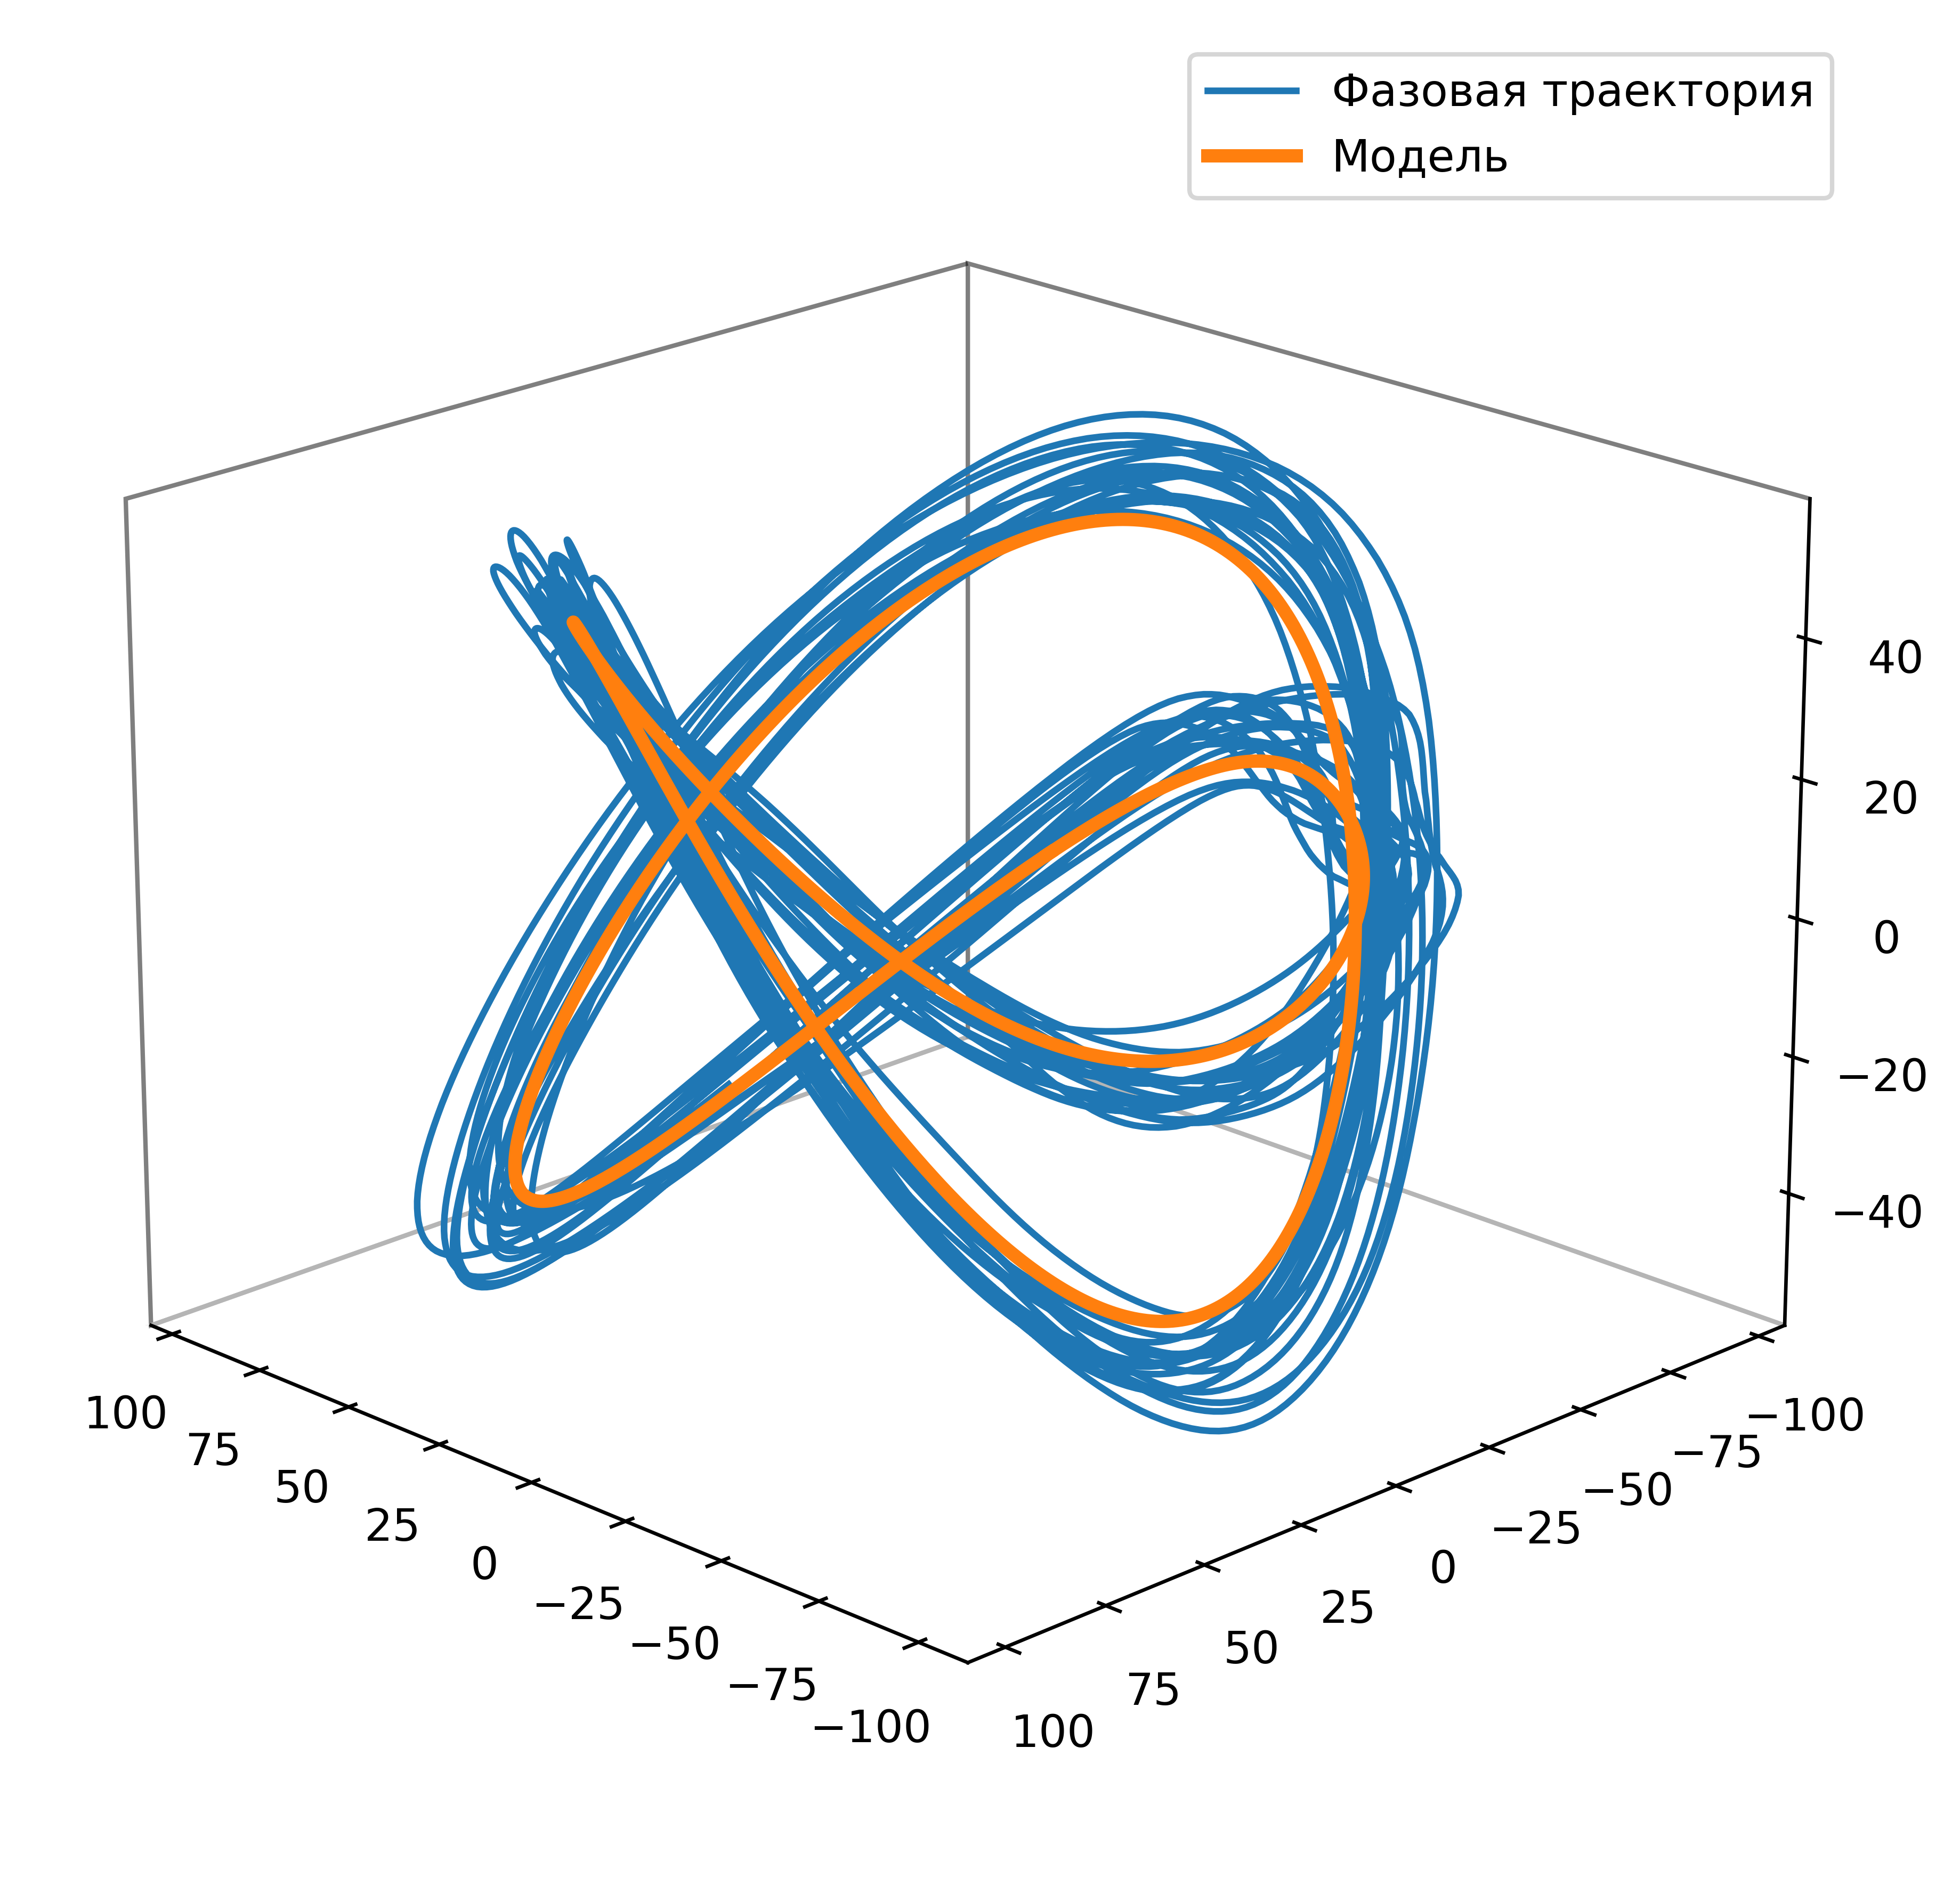
\includegraphics[width=0.55\textwidth]{st2.jpg}}
% 	    %\includegraphics[width=0.5\linewidth]{error.jpg}
% 	    \caption{Квазипериодический временной ряд и его фазовая траектория.}
%     \end{figure}
    
% Выбранны главные компоненты $\mathbf{y}_1,\dots,\mathbf{y}_p$, аппроксимирующие фазовую траекторию. Будем полагать, что они нормированны. В собственном пространстве размерности $p$ фазовая траектория не имеет самопересечений с точностью до среднеквадратичного отклонения. Будем рассекать фазовую траекторию гиперплоскостью, наиболее приближенной к плоскости симметри фазовой траектории. Для нахождения плоскости симметрии воспользуемся методом, описанным в \cite{karkishchenko2013recovery, karkishchenko2013reflective}. Пусть $y_1 = 0$ совпадает с плоскостью симметрии. Для множества точек $(\mathbf{y_1}, \dots, \mathbf{y_p})$ вводитя вспомогательный вектор $Y = [\mathbf{y_1}^{\mathsf{T}}, \dots, \mathbf{y_p}^{\mathsf{T}}]^{\mathsf{T}}$. Тогда вектор $Y_s$, соответствующий симметричному множеству точек, минимизирующий отклонение $\| Y_s - Y  \|_2$, получается из $Y$ посредством линейного преобразования
%     \[ Y_s = QY. \]
% Тогда в качестве рассекающей гиперплоскости будем выбирать ту, которая минимизирует отклонение
%     \[ \| \tilde{Y}_s - \tilde{Y} \|_2. \]
% Вектор $\tilde{Y}$ состоит из компонент вектора $Y$ в системе координат, повернутой вокруг начала отсчета таким образом, чтобы ось $y_1$ была совмещена с нормалью, задающей гиперплоскость.

% \section{Сечение фазовой траектории в пространстве оптимальной размерности}
%     Требуется провести секущую гиперплоскость в собственном пространстве, разбивающую фазовую траекторию на сегменты, соответствующие полупериодам временного рядя \eqref{ts}. Предлагаемый алгоритм является обобщением метода, предложенного в работе \cite{motrenko2015extracting}. Сечение фазовой траектории происходит в пространстве размерности больше, чем два.
    
%     Выбирается произвольная точка $ x(k_0)$ временного ряда \eqref{ts}. Ее фаза полагается равной нулю. Пусть $\mathbf{h_0}$ -- направляющий вектор из начала координат в выбранную точку на фазовой траектории.  Сроится касательная к фазовой траектории в выбранной точке. Пусть $\mathbf{a}$ -- направляющий вектор касательной. Проводится гиперплоскость через выбранную точку и начало координат (главные компоненты полагаем нормированными). По касательной выбирается вектор нормали к гиперплоскости
%         \[ \mathbf{n} = \mathbf{a} - \pi_{\mathbf{h_0}}(\mathbf{a}).\]
%     Уравнение секущей гиперплоскости
%         \[ (\mathbf{y} - \mathbf{h_0},\, \mathbf{n}) = 0. \]
%     Уравнение прямой с направляющим вектором $\mathbf{h_0}$ в параметрической форме
%         \[ \mathbf{y} = t\mathbf{h_0},\quad t\in\mathbb{R}. \]
%     Точки пересечения фазовой траектории с гиперплоскостью наносятся на исходный временной ряд. Ожидается, что если пересечение произошло ближе, чем половина от максимального размаха траектории, то точка имеет фазу, равную нулю. Если же пересечение произошло дальше, чем половина от максимального размаха траектории, то ожидается точка с фазой, равной $\pi$.
    
%     \begin{figure}[h!]\label{fig4}
% 	    \center{\includegraphics[width=0.5\linewidth]{slide_5}}
% 	    \caption{Сечение фазовой траектории.}
%     \end{figure}
    
% \newpage
    

    
%   \begin{figure}[ht]\label{fig8}
% 	    \center{\includegraphics[width=1\linewidth]{newplot.jpg}}
% 	    \caption{Результат алгоритма сегментации.}
%     \end{figure}  
    
% \newpage

% % \section{Анализ ошибки}
% % \emph{Дана выборка. Рисунок с разметкой на фазу и полуфазу. Тест -- другой временной ряд с аналогичным типом движения. С помощью PCA переходим в пространство размерности 2. Итеративно увеличиваем размерность пространства, пока точность классификации не станет максимальной. Классификатор -- линейный SVM.}

% % \emph{Оценка параметров гиперплоскости с помощью бустрапа - ?}

% % \emph{График качества классификации в зависимости от размерности.}

% % \emph{Смотрим на качество уменьшения и восстановления другого временного ряда и ряда с размеченной выборкой.}

% % \emph{Возможно:
% % 1) поиграться с марджином в размерности на 1 больше, на 1 меньше и в самой оптимальной.
% % 2) проверить, что прямая, соединяющаяся размеченные точки, перпендикулярна гиперплоскости, построенной SVM.
% % 3) можно посмотреть на зависимость уверенности (адекватности разделимости) SVM от размерности.}




% %%%% если имеется doi цитируемого источника, необходимо его указать, см. пример в \bibitem{article}
% %%%% DOI публикации, зарегистрированной в системе Crossref, можно получить по адресу http://www.crossref.org/guestquery/

% %%%% если имеется doi цитируемого источника, необходимо его указать, см. пример в \bibitem{article}
% %%%% DOI публикации, зарегистрированной в системе Crossref, можно получить по адресу http://www.crossref.org/guestquery/.

\bibliographystyle{unsrt}
\bibliography{biblio}


\end{document} 